\documentclass[12pt,a5]{bxjsarticle}

\usepackage{xltxtra}
\setmainfont{IPAPMincho}
\setsansfont{IPAPGothic}
\setmonofont{IPAGothic}
\XeTeXlinebreaklocale "ja"

\usepackage{hyperref}
\usepackage{listings}
\usepackage{verbatim}

\newcommand{\e}{\mathrm{e}}

\title{物理学情報処理論2 problem1}
\date{}

\begin{document}
\maketitle

Euler法による$ \frac{\mathrm{d}y(x)}{\mathrm{d}x} = \exp(-y(x)), y(0) = 1 $ の結果と真値との差は以下のようになり、
両対数グラフで直線になっている。
つまり、この直線の傾きを$ \alpha $とすると、真値との差は$ O(\mbox{時間刻み}^\alpha) $程度となることがわかる。

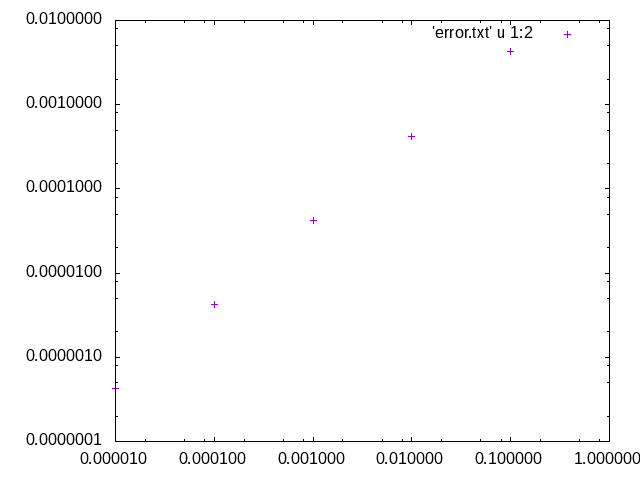
\includegraphics[width=\linewidth]{error.png}

誤差を時間刻みで割った値(error.txtの3列目に出すようなプログラムを書いた)は、
たしかに$ \frac{1}{2(1+\e)} \ln(\frac{1+\e}{\e}) $へと近づいている。

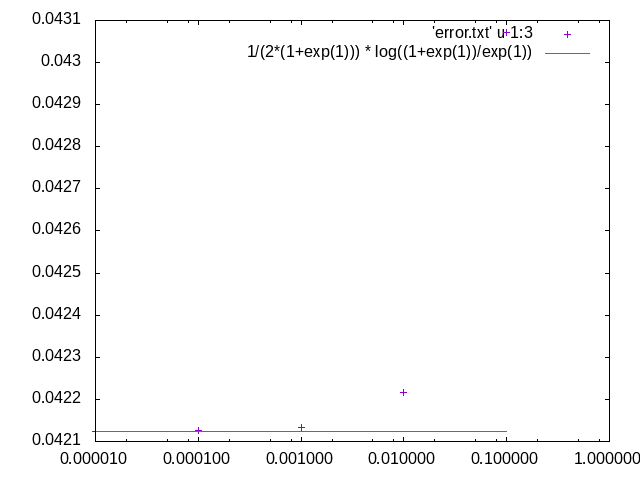
\includegraphics[width=\linewidth]{error-per-delta.png}

以下のスクリプトを用いて、error.txtから図を生成した。
\lstinputlisting[caption=plot.sh]{plot.sh}

\end{document}
